%%%%%%%%%%%%%%%%%%%%%%%%%%%%%%%%%%%%%%%%%%%%%%%%%%%%%%%%%%%%%%%%%%%%%%%%%%%%%%%%%%%%%%%%%%%%%%%%%%%%
% ==================================================================================================
% --------------------------------------------------------------------------------------------------
\chapter{Implementation}
This appendix contains implementation details.
%%%%%%%%%%%%%%%%%%%%%%%%%%%%%%%%%%%%%%%%%%%%%%%%%%%%%%%%%%%%%%%%%%%%%%%%%%%%%%%%%%%%%%%%%%%%%%%%%%%%
\section{Computing}
All computation in the current work was performed using the following workstation and software:
\begin{itemize}[topsep=0pt,itemsep=-6pt]
  \item \textbf{CPU:} Intel Core i7-6700K 4.00 GHz
  \item \textbf{RAM:} 16.0 GB DDR4
  \item \textbf{GPU:} NVIDIA GeForce GTX 980 Ti
  \item \textbf{OS:} Windows 10
  \item \textbf{Code:} Matlab R2011a
\end{itemize}
%%%%%%%%%%%%%%%%%%%%%%%%%%%%%%%%%%%%%%%%%%%%%%%%%%%%%%%%%%%%%%%%%%%%%%%%%%%%%%%%%%%%%%%%%%%%%%%%%%%%
\section{Manual Segmentations}
It was necessary to create and edit a small number of binary segmentation masks during this work.
To do this, the Editor module from the 3D Slicer imaging platform~\cite{Fedorov2012} was used,%
\footnote{3D Slicer Editor tool documentation is available here:\\
  \hreftt{https://www.slicer.org/wiki/Documentation/4.6/Modules/Editor}.}
including the Wand, Paint, and Erase functions.
Figure~\ref{fig:m08-rev-slicer} shows the user interface during a lesion segmentation.
\begin{figure}[ht]
  \centering
  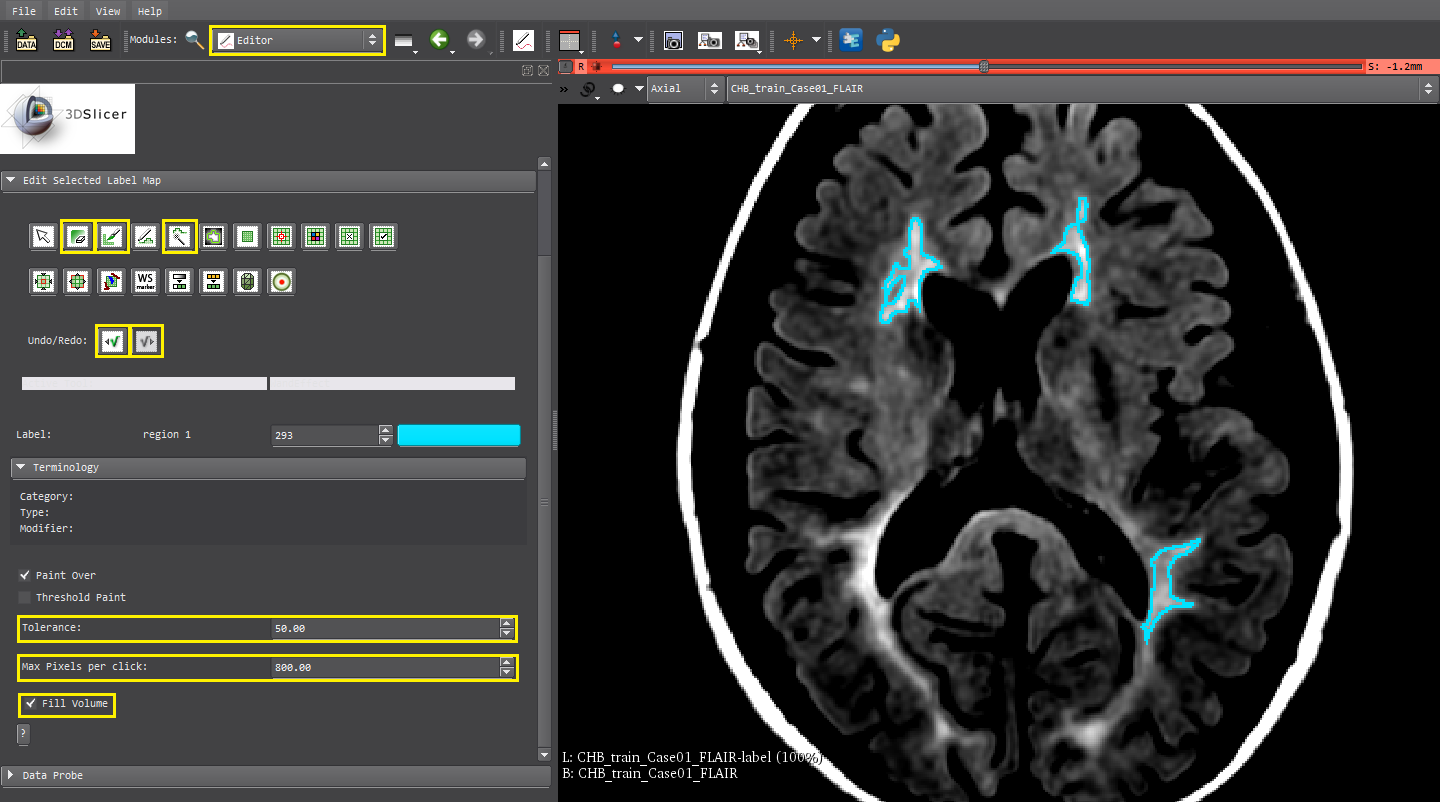
\includegraphics[width=\textwidth]{m08rev-slicer.png}
  \caption{3D Slicer user interface for performing in-house manual segmentations and revisions.
    The tools used are highlighted in yellow, while the in-progress segmentation is shown in blue.
    Best viewed in colour.}%
  \label{fig:m08-rev-slicer}
\end{figure}
% ==================================================================================================
\subsection{MS 2008 WMH Masks}\label{ss:m08-rev}
Since the reported performance of an automatic segmentation algorithm depends on
the manual segmentations to which it is compared,
it is important to obtain good manual segmentations.
Unfortunately, the original manuals in the MS 2008 Segmentation Challenge
contained obvious artifacts and inconsistencies,
as shown at left in Figure~\ref{fig:m08-rev}.
Therefore, it was deemed necessary to redo these manuals.
The resulting revisions are shown at right in Figure~\ref{fig:m08-rev}.
\begin{figure}
  \centering
  \begin{minipage}{6cm}
    \begin{subfigure}{\textwidth}
      \centering\subcaption{Original}%
      \label{fig:m08-rev-o}
      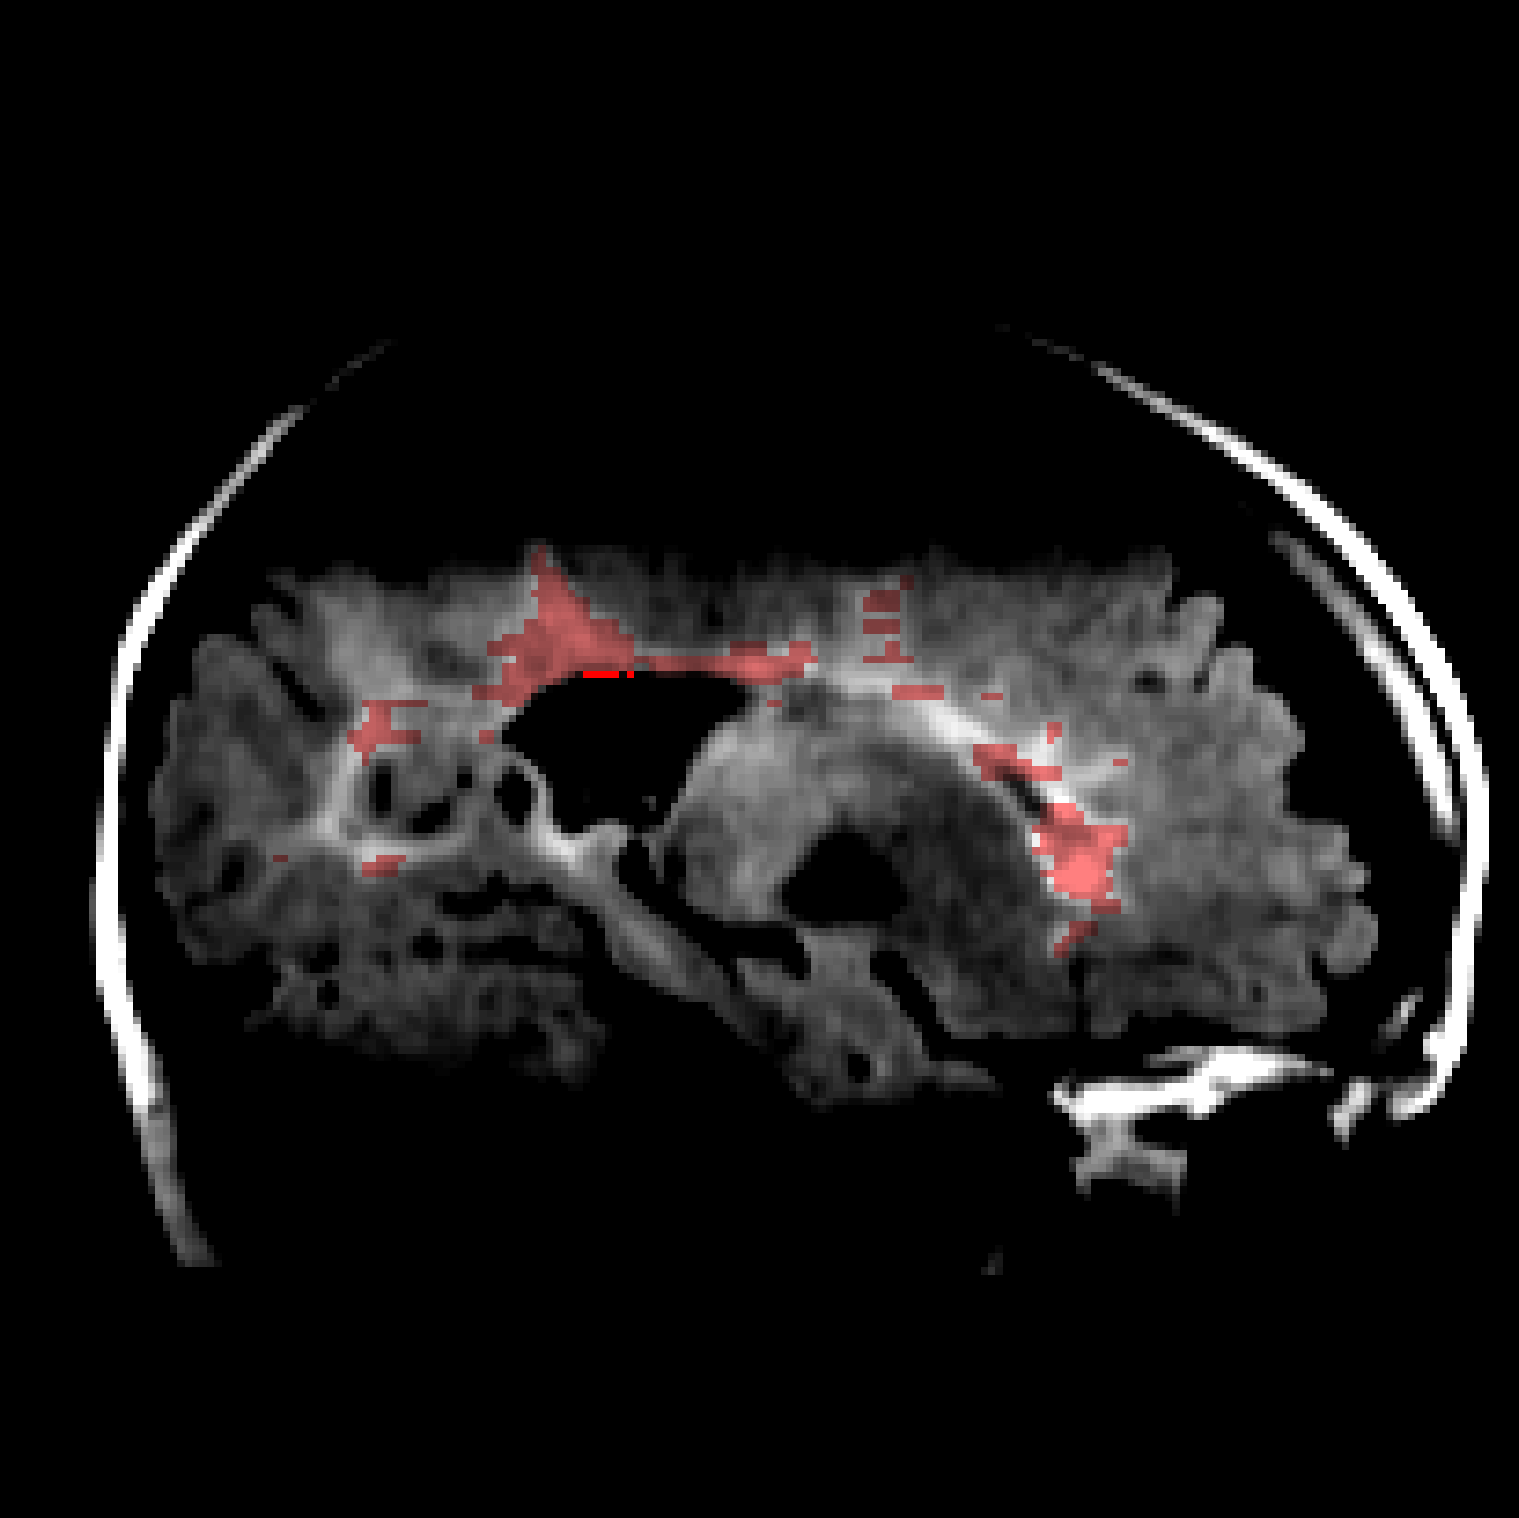
\includegraphics[height=6cm]{m08rev-01-d2-z146-o}\\[0.2em]
      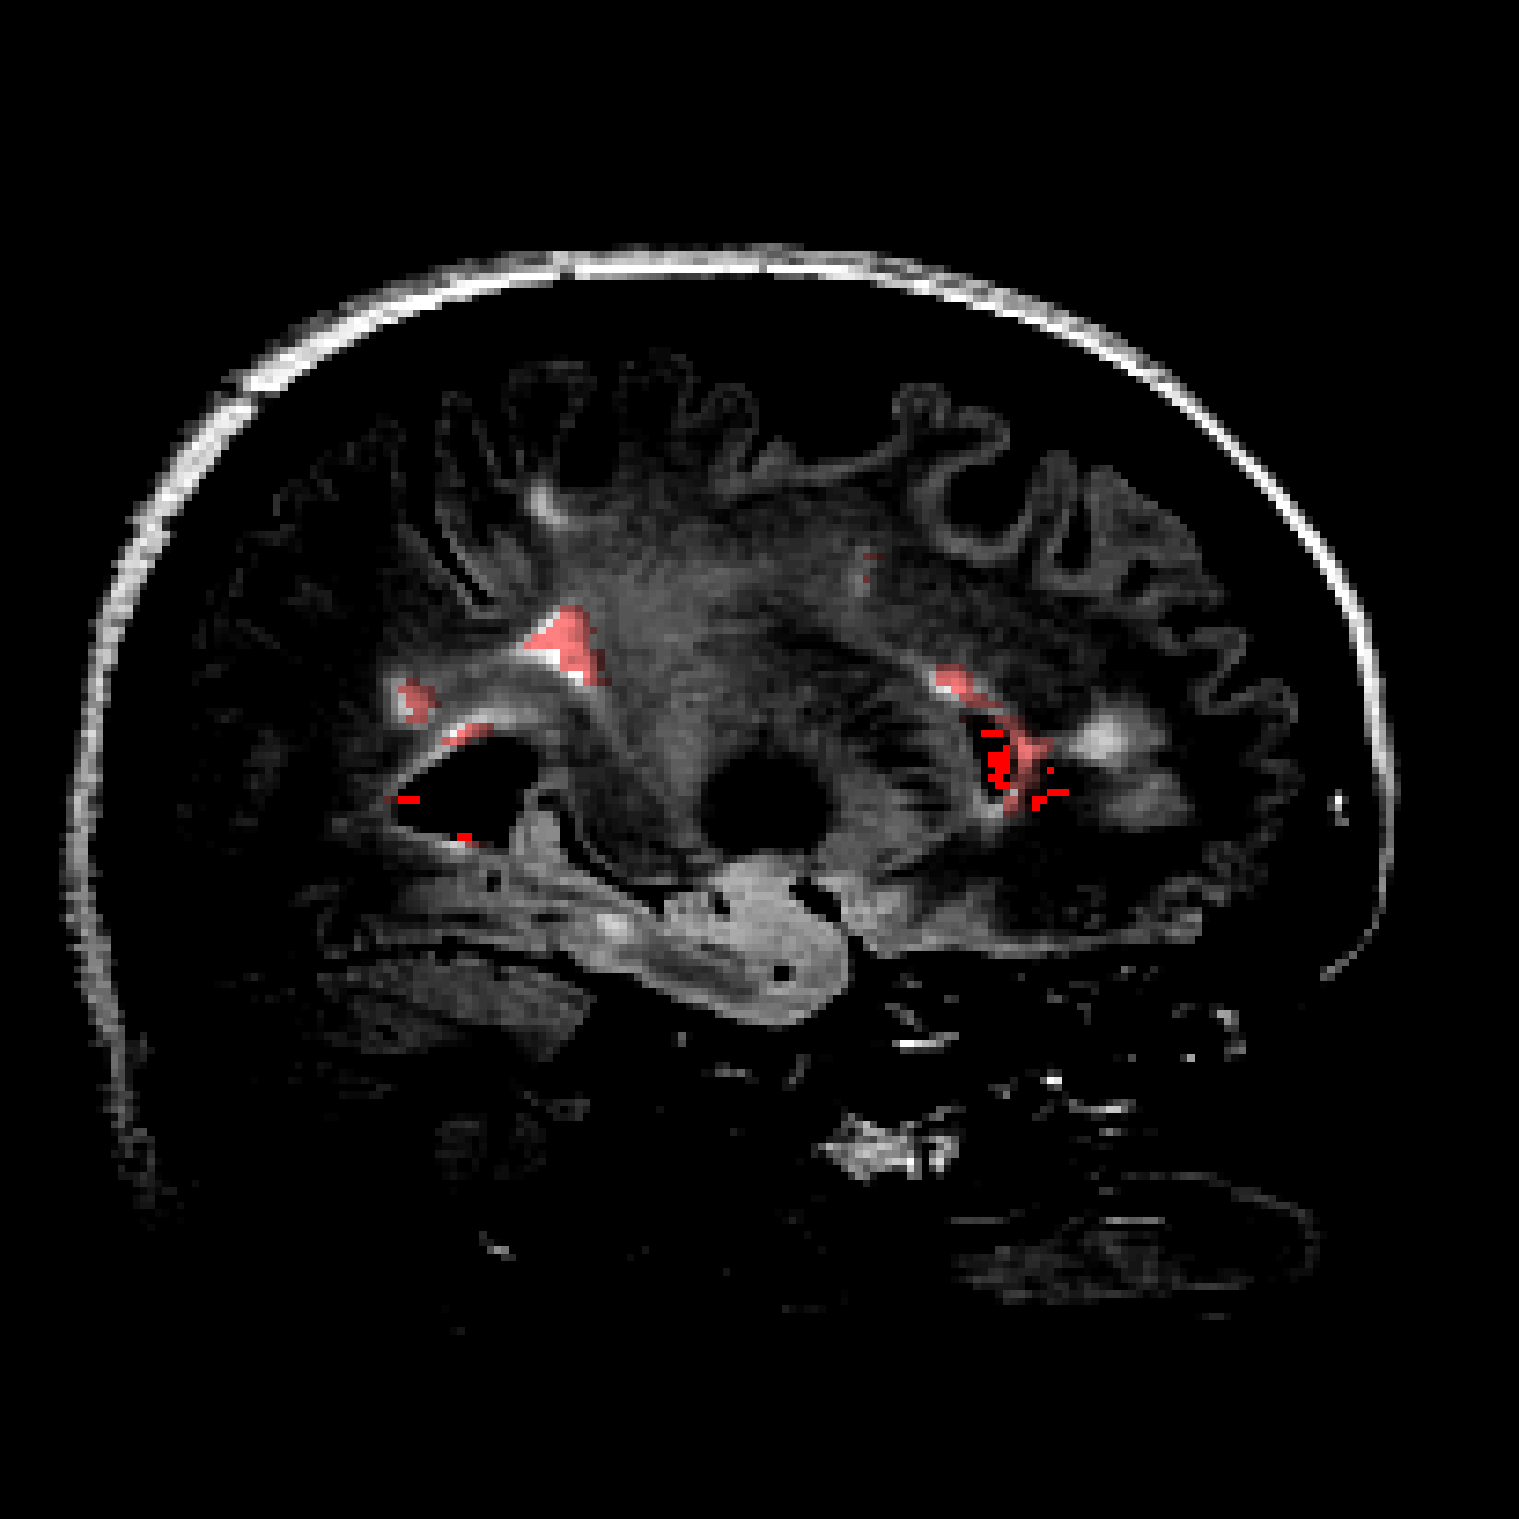
\includegraphics[height=6cm]{m08rev-05-d2-z107-o}\\[0.2em]
      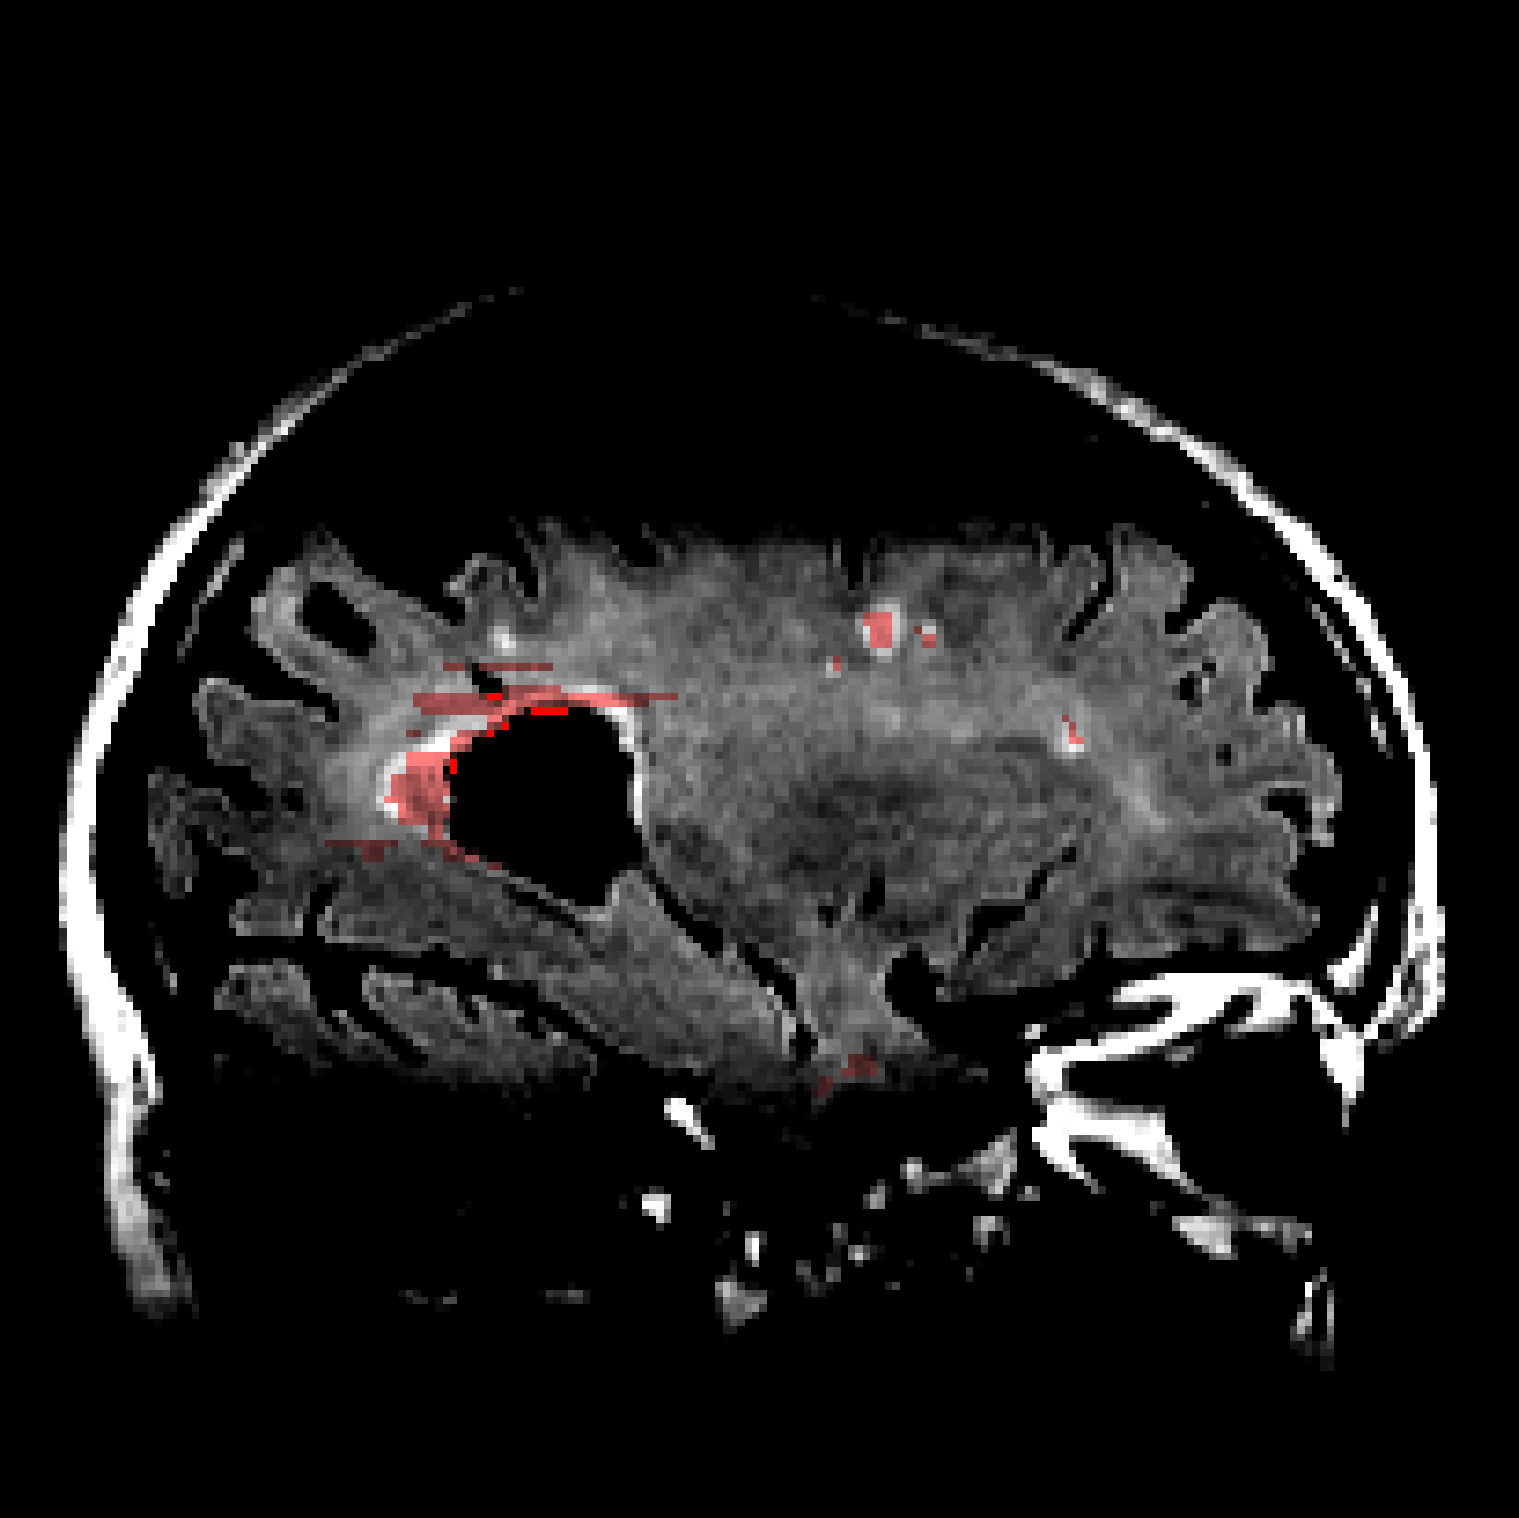
\includegraphics[height=6cm]{m08rev-06-d2-z101-o}
    \end{subfigure}
  \end{minipage}
  \begin{minipage}{6cm}
    \begin{subfigure}{\textwidth}
      \centering\subcaption{Revision}%
      \label{fig:m08-rev-r}
      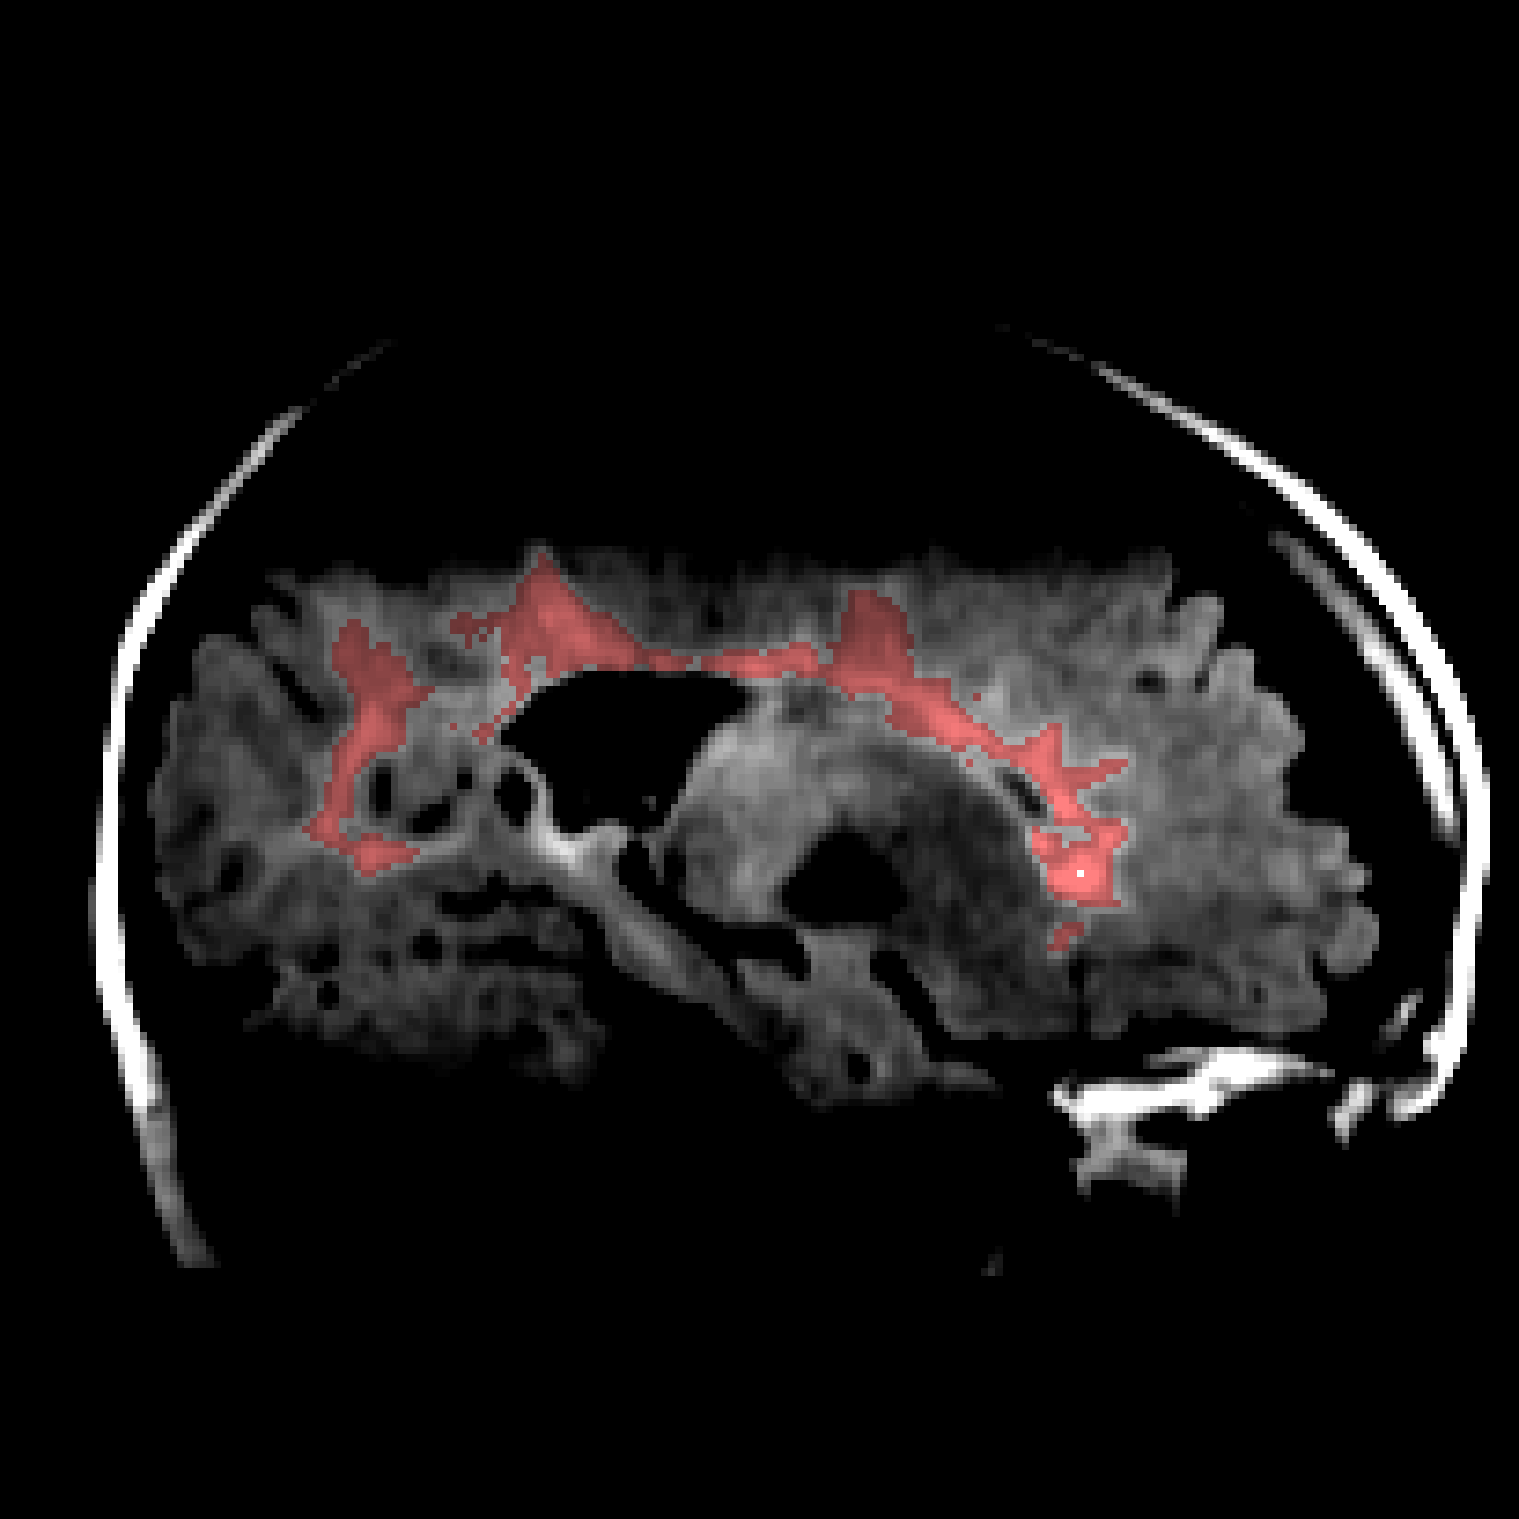
\includegraphics[height=6cm]{m08rev-01-d2-z146-r}%
      \makebox[0pt][r]{\textcolor{white}{\raisebox{0.5em}{ CHB 01 }}}\\[0.2em]
      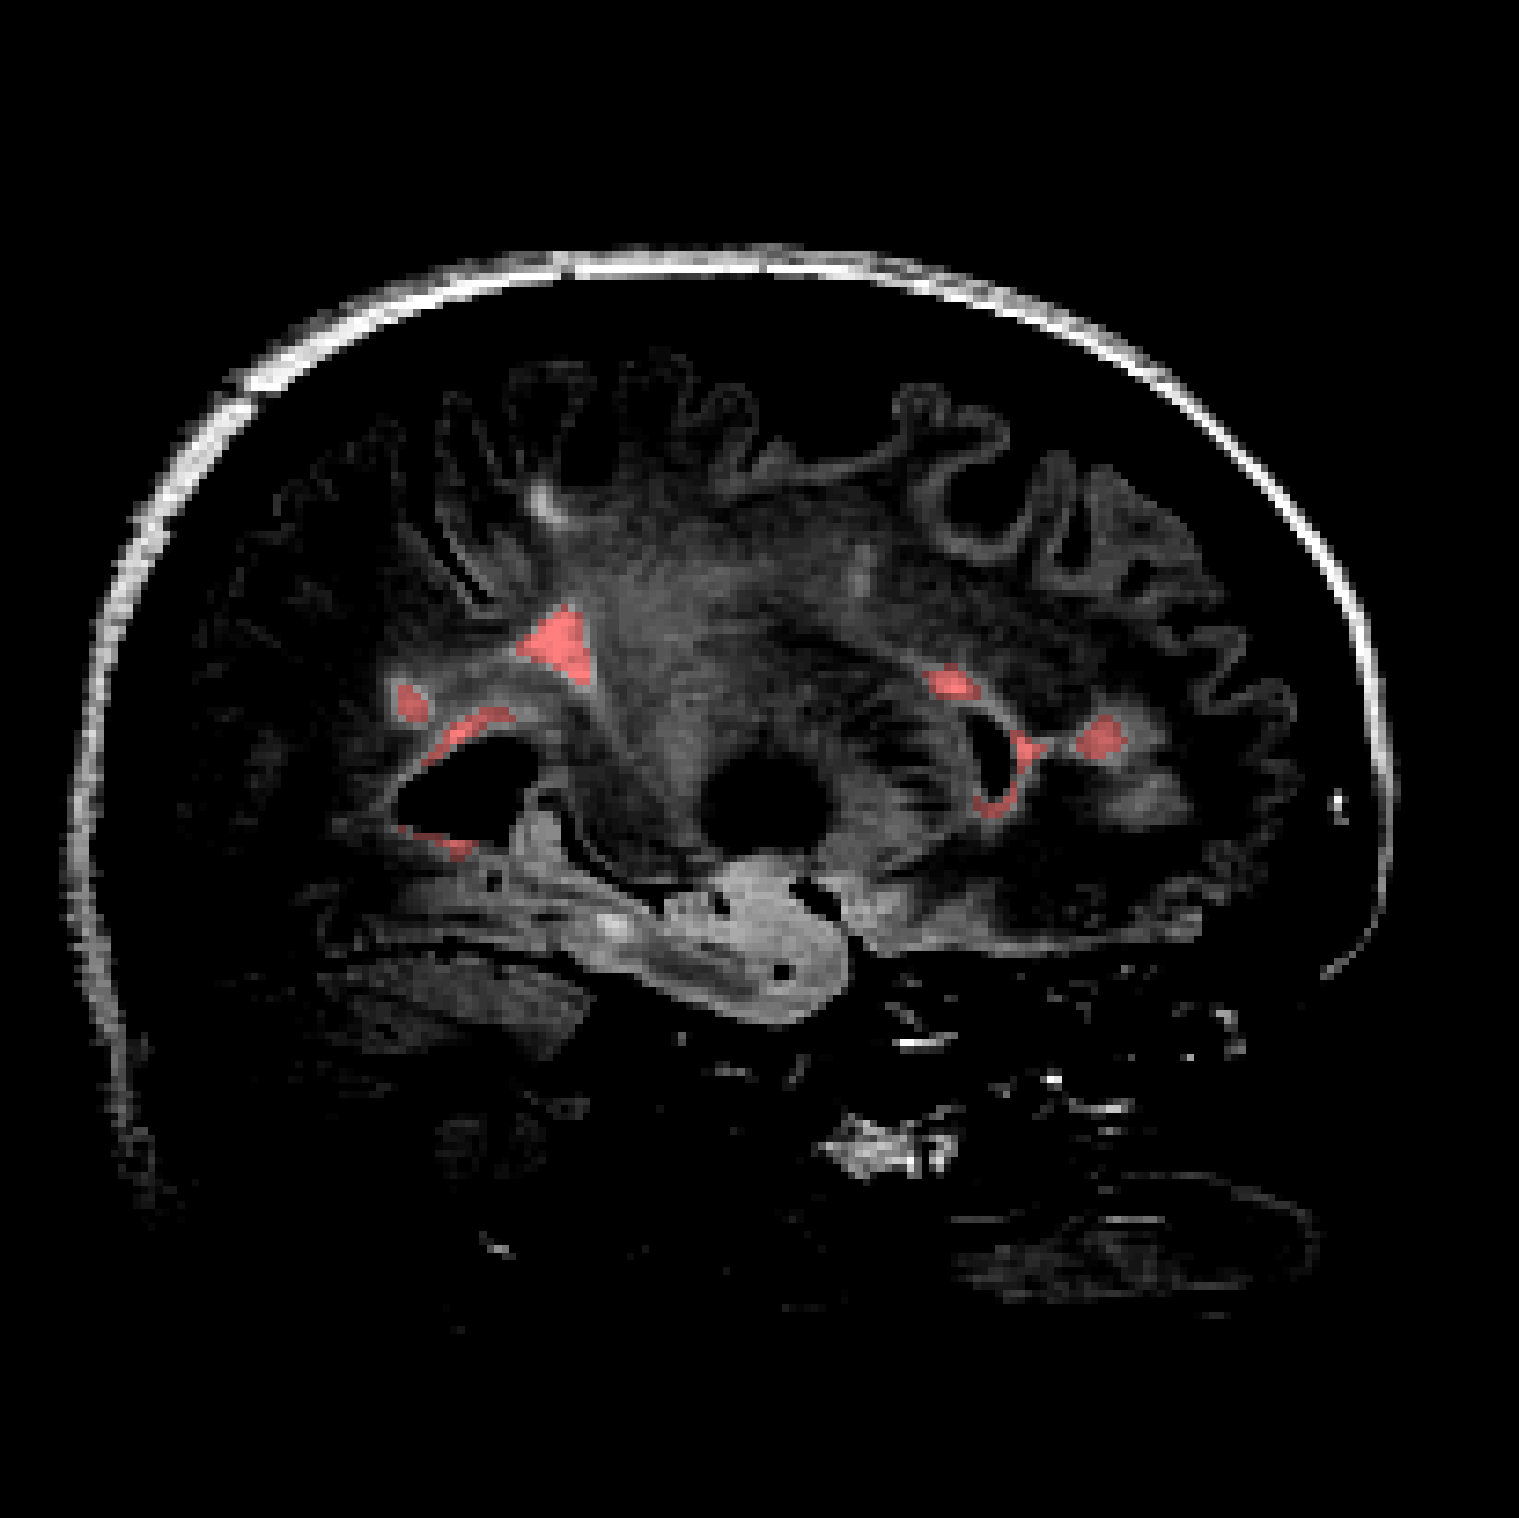
\includegraphics[height=6cm]{m08rev-05-d2-z107-r}%
      \makebox[0pt][r]{\textcolor{white}{\raisebox{0.5em}{ CHB 05 }}}\\[0.2em]
      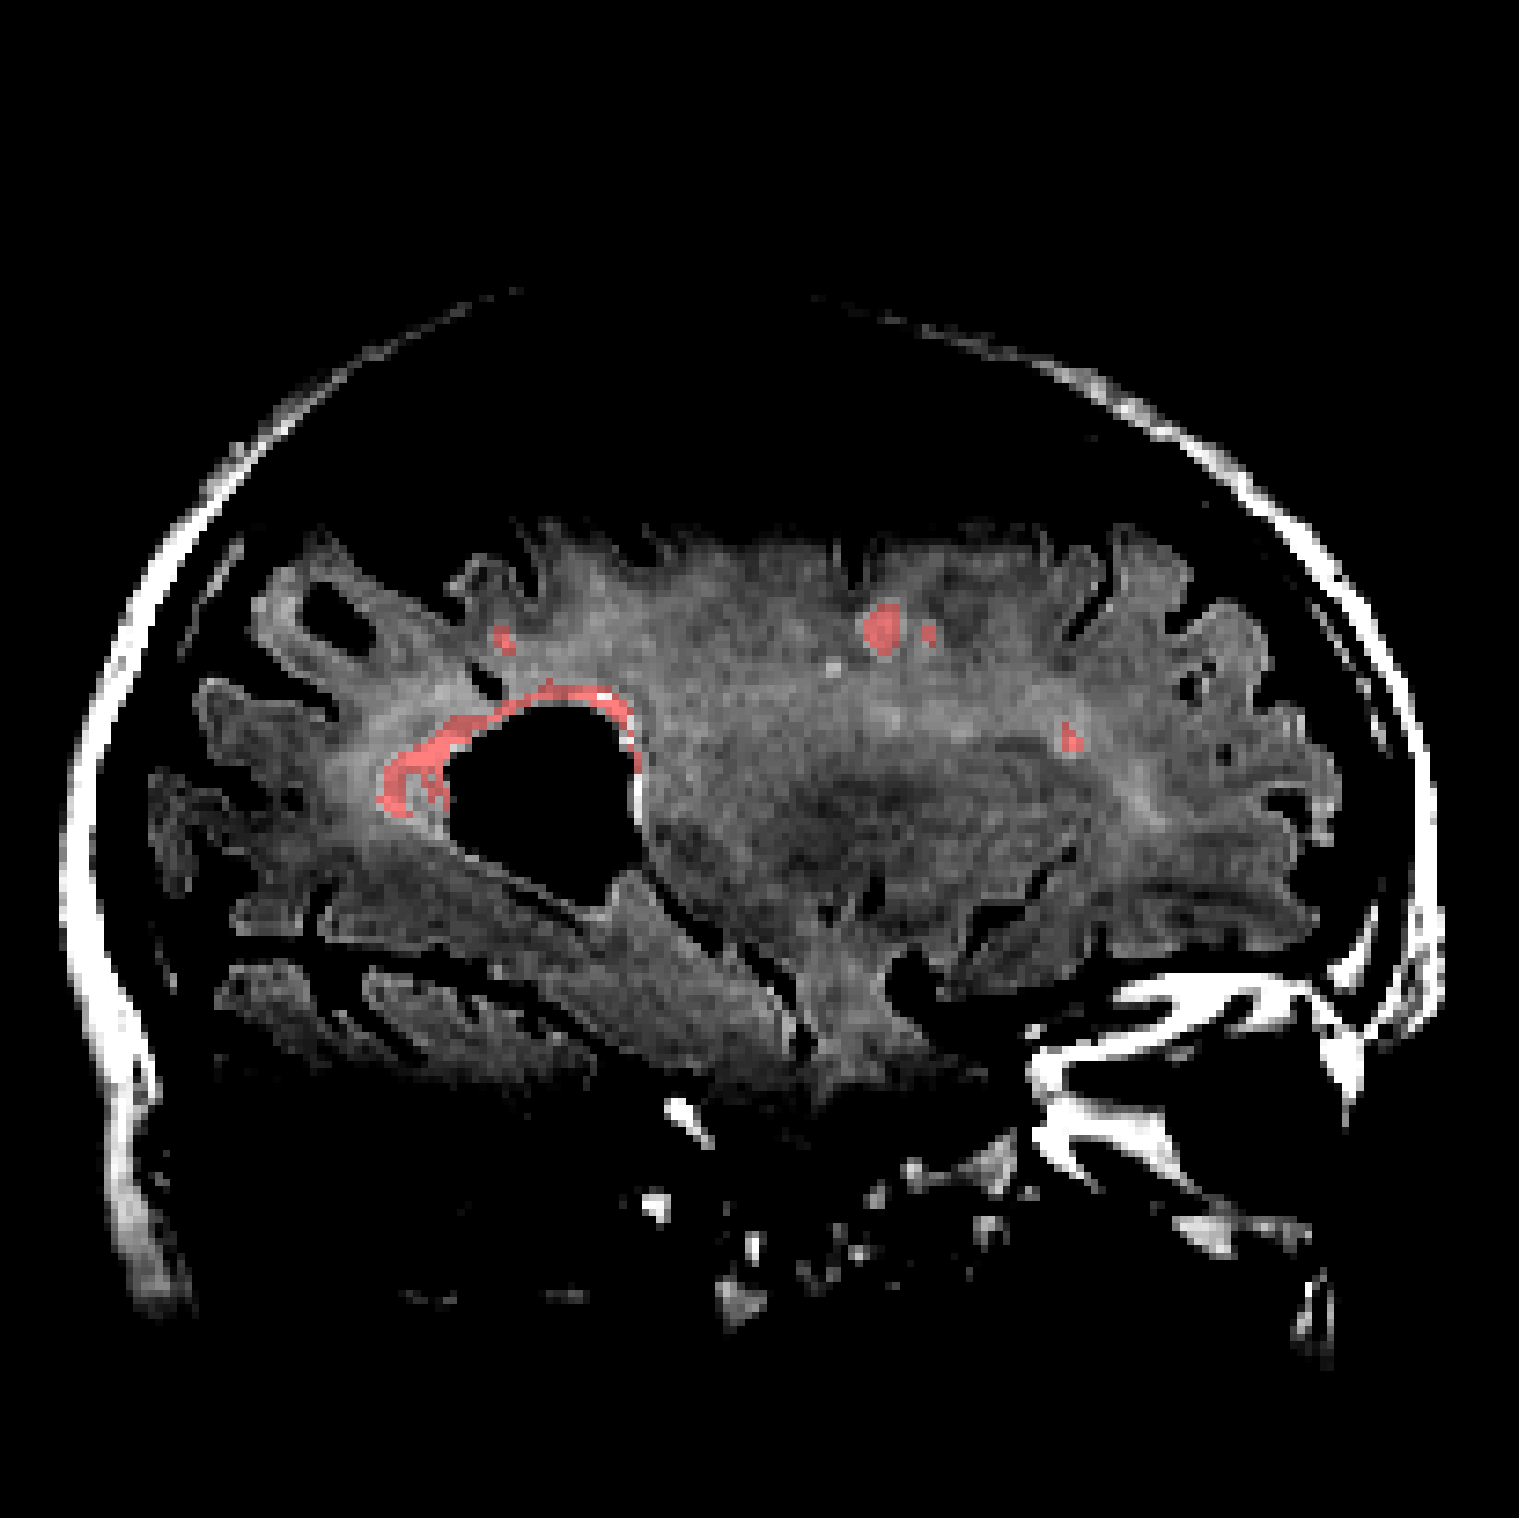
\includegraphics[height=6cm]{m08rev-06-d2-z101-r}%
      \makebox[0pt][r]{\textcolor{white}{\raisebox{0.5em}{CHB 06 }}}
    \end{subfigure}
  \end{minipage}
  \caption{Example revisions to the manual segmentations for the MS 2008 challenge dataset.
  Best viewed in colour.}%
  \label{fig:m08-rev}
\end{figure}
% ==================================================================================================
\subsection{Brain Mask}\label{ss:brainmask}
In order to vectorize image data for parallel processing,
a binary mask selecting voxels of interest in standardized space is also required.
Since only voxels in the brain are of interest, this mask is called a ``brain mask''.
The brain mask used here was derived from
the ICBM tissue prior images~\cite{Mazziotta2001} in MNI space:
after initial thresholding of the combined $\gm{}+\wm{}+\csf{}$ probabilities at 0.5,
manual refinements were completed and symmetry was enforced.
The mask is slightly small on purpose,
since tissues outside the brain are frequently bright in FLAIR images,
and can be mistaken for lesions by naive models.
The resulting mask is shown in Figure~\ref{fig:brainmask}.
\begin{figure}
  \centering
  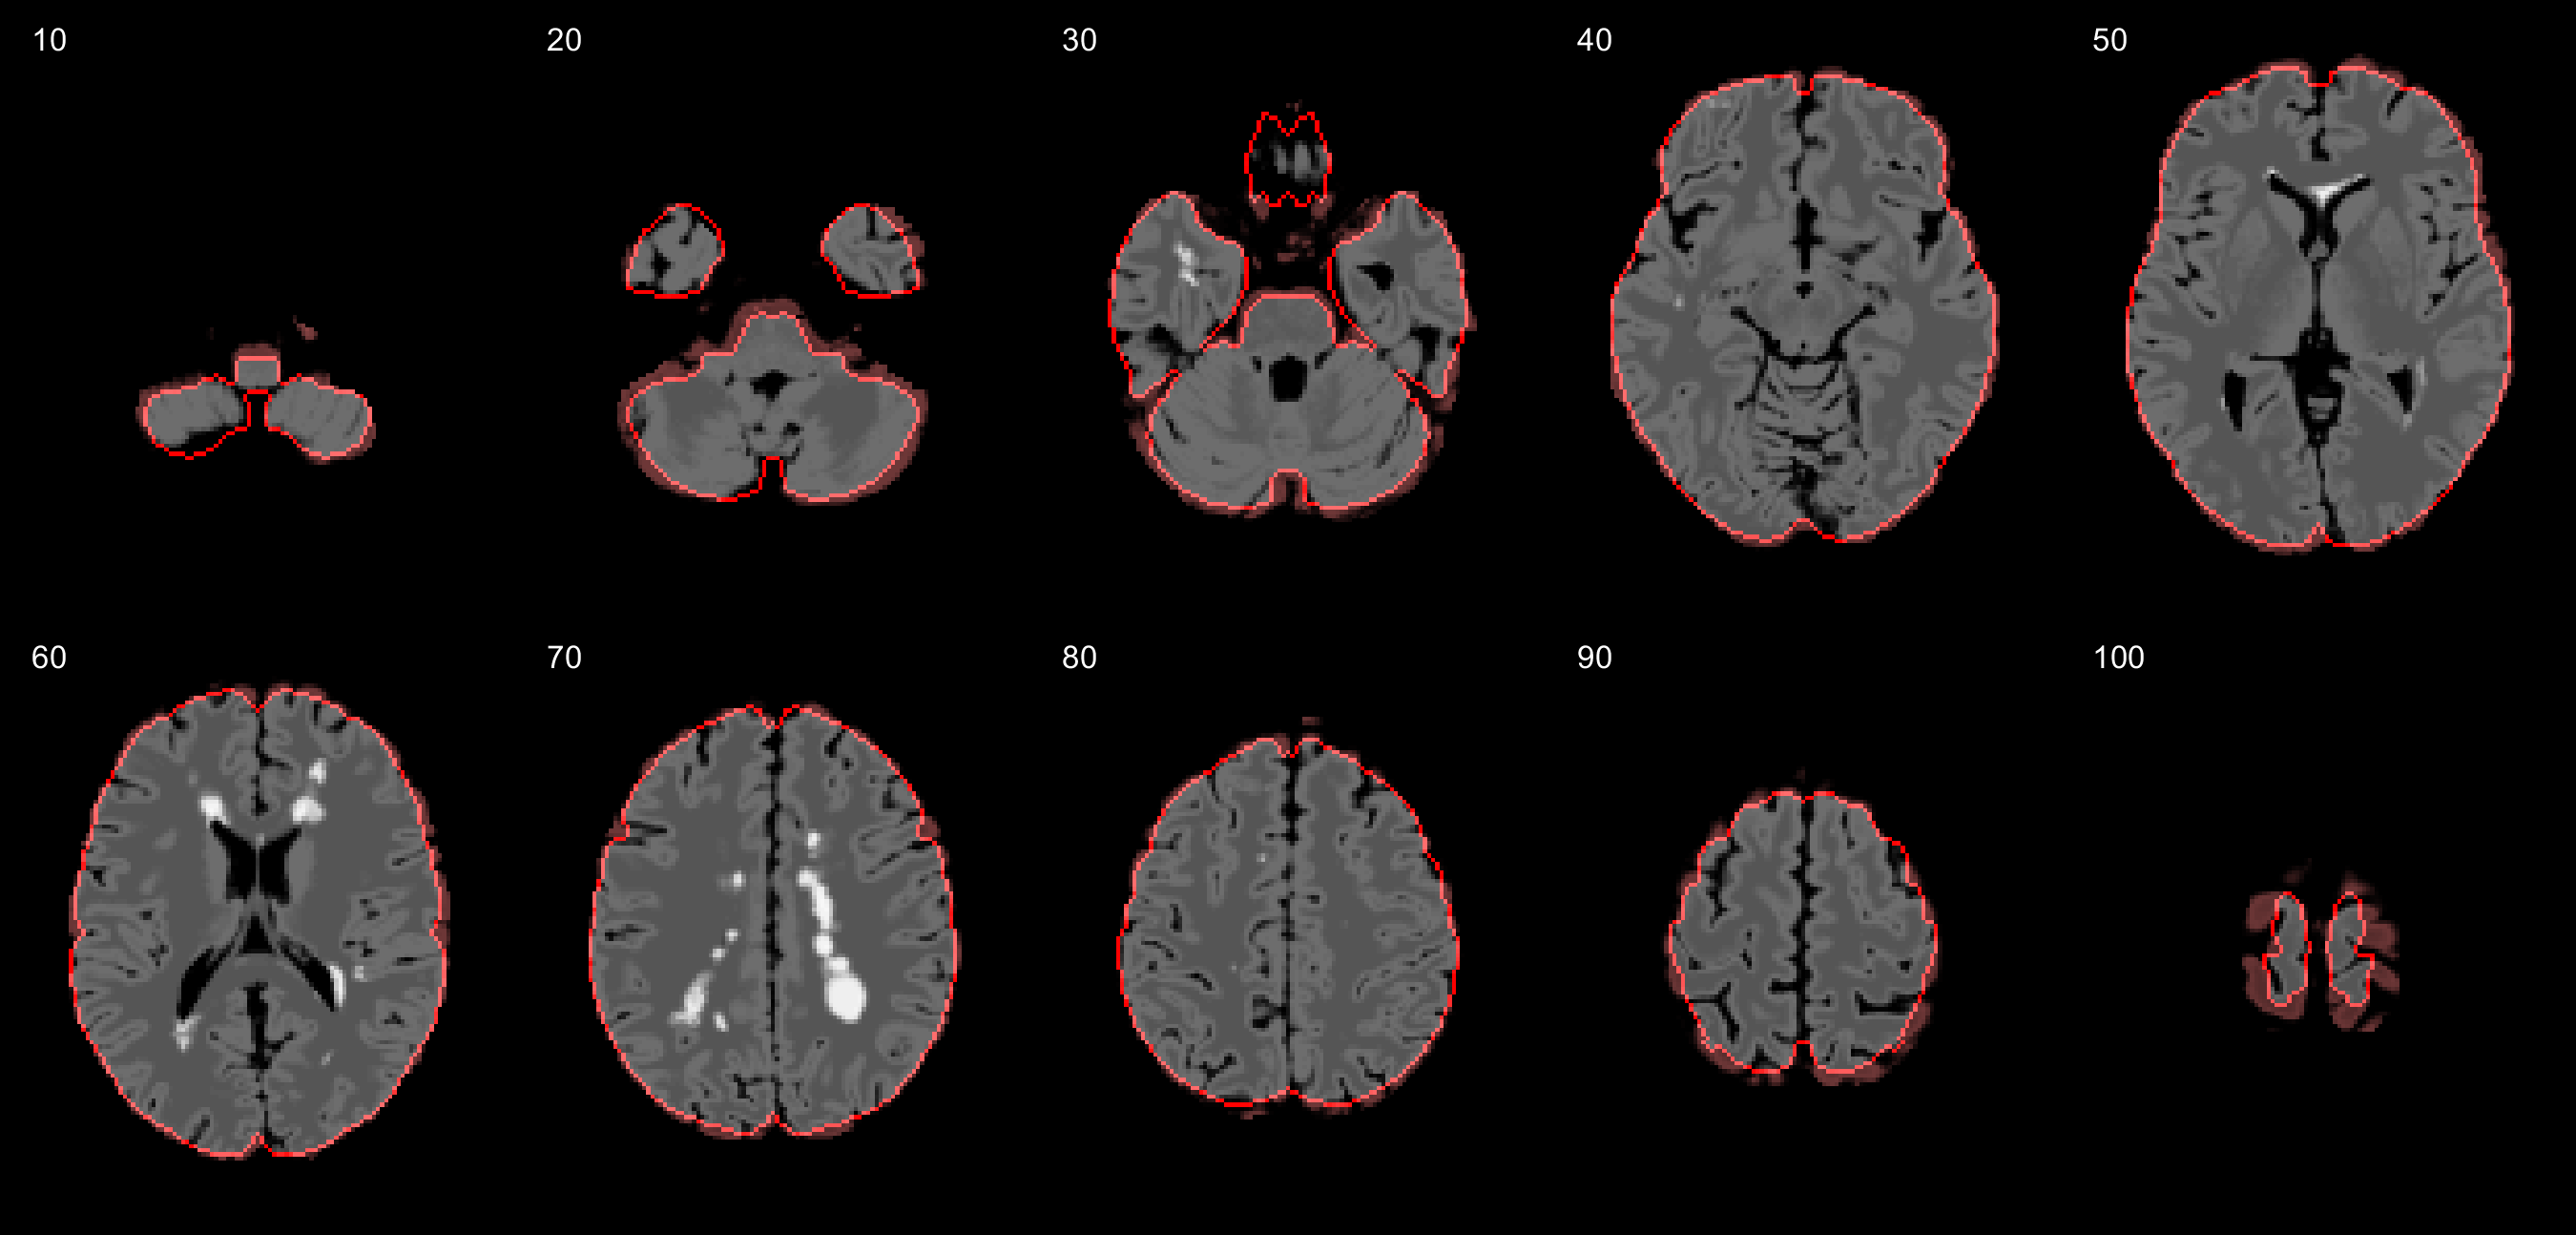
\includegraphics[height=2\sliceheight]{brainmask.png}
  \caption{Manually refined brain mask in MNI space, overlaid on a simulated BrainWeb FLAIR image.
    Mask outline is highlighted in red; inclusions are shown in grayscale; exclusions tinted red.
    Best viewed in colour.}%
  \label{fig:brainmask}
\end{figure}
%%%%%%%%%%%%%%%%%%%%%%%%%%%%%%%%%%%%%%%%%%%%%%%%%%%%%%%%%%%%%%%%%%%%%%%%%%%%%%%%%%%%%%%%%%%%%%%%%%%%
\section{Acceleration}
Speed of model fitting is a significant factor during development,
particularly considering optimization of hyperparameters.
Faster training yields more model iterations, which inevitably bear improvements.
This section summarizes the implementation decisions
specifically taken to accelerate training and testing of the model.
% ==================================================================================================
\subsection{Parallel Model Estimation}\label{s:parallelfit}
While the estimation procedure outlined in \S~\ref{ss:modelfitting}
must be repeated for all standardized voxels in the brain mask,
it is possible to do this in parallel, since every estimation is independent.
To do so, the training data must first be vectorized with respect to spatial location $x$,
and matrix operations expanded explicitly to accommodate the new dimension.
\par
% __JK__ add some details about gpuArray in Matlab?
To begin, the standardized training data from all subjects
-- features $\tilde{\bm{\Y}}_{\gamma}(x)$, with $\tilde{\Y}_{\gamma}^{\et0}=1$,
and labels $\C_{\gamma}(x)$ --
are sampled from nonzero locations in the brain mask $M(x)$.
These data are stored in two matrices $\vox{Y}$ and $\vox{C}$,
with dimensions $[X,N,K+1]$ and $[X,N,1]$, respectively, where
$X$ is the total number of nonzero voxels in the brain mask,
$N$ is the number of subjects, and
$K$ is the number of features.
A similar matrix is constructed for the initial parameters $\bb^{(0)}(x)$, denoted $\vox{B}^{(0)}$,
with dimensions $[X,1,K+1]$.
Let $\vox{Y}_n^k$ denote the vector of data
from all voxels for the $k$\ss{th} feature from the $n$\ss{th} subject,
and so on for $\vox{C}$ and $\vox{B}$.
\par
In order to simplify subsequent calculations,
the feature data are rectified according to the class labels,
before the first iteration, as in
\begin{equation}
  \vox{Y}_n^k =
  \begin{cases}
    +\vox{Y}_n^k, & \vox{C}_n \ge 0.5\\
    -\vox{Y}_n^k, & \vox{C}_n  <  0.5\\
  \end{cases},\qquad\forall\et k \in \{1,\dots,K\}.
\end{equation}
Next, for a given iteration $t$, the following vector-compatible expansions of Equations
(\ref{eq:llgradient}), (\ref{eq:llhessian}), and (\ref{eq:newtonmap})
yield the desired update matrix $\Delta\vox{B}^{(t)}$.
%These calculations are performed in \nameref{m:vlrmap.m}.
Regarding notation:
1.\ the iteration index ${}^{(t)}$ is omitted for clarity,
2.\ element-wise multiplication is denoted by $\circ$, and
3.\ the variable $K$ is now defined as $1$, since this is essential to the simplification.
\par
\begin{align}
  \vox{S} &= \frac{1}{1+e^{+\eta}},\qquad \eta = \vox{B}^0 + \left(\vox{B}^1\ep\vox{Y}^1\right)\\
  \vox{A} &= \vox{S}\ep\left(1-\vox{S}\right)\\
  \vox{G} &= \nabla_{\vox{B}}\L - \lambda\vox{B} \nonumber\\
          &= \left[\begin{array}{c}
               \vox{G}^0 \\
               \vox{G}^1
             \end{array}\right] \nonumber\\
          &= \left[\begin{array}{c}
               \sum_{n=1}^{N}\left( \vox{Y}_n^0\ep\vox{S} \right) \\
               \sum_{n=1}^{N}\left( \vox{Y}_n^1\ep\vox{S} \right)
             \end{array}\right]
           - \lambda\left[\begin{array}{c}
               \vox{B}^0 \\
               \vox{B}^1
             \end{array}\right] \\
  \vox{H} &= \nabla_{\vox{B}}^1\L -\lambda\vox{I} \nonumber\\
          &= \left[\begin{array}{cc}
               \vox{H}^{0,0} & \vox{H}^{0,1} \\
               \vox{H}^{1,0} & \vox{H}^{1,1}
              \end{array}\right] \nonumber\\
          &= \left[\begin{array}{cc}
               \sum_{n=1}^{N}\left( \vox{A}\ep\vox{Y}_n^0\ep\vox{Y}_n^0 \right) &
               \sum_{n=1}^{N}\left( \vox{A}\ep\vox{Y}_n^1\ep\vox{Y}_n^0 \right) \\
               \sum_{n=1}^{N}\left( \vox{A}\ep\vox{Y}_n^0\ep\vox{Y}_n^1 \right) &
               \sum_{n=1}^{N}\left( \vox{A}\ep\vox{Y}_n^1\ep\vox{Y}_n^1 \right)
             \end{array}\right] - \lambda\left[\begin{array}{cc} 1 & \\ & 1\end{array}\right]\\
  \vox{D} &= \det{\vox{H}} \nonumber\\
          &= \left(\vox{H}^{0,0}\ep\vox{H}^{1,1}\right)
           - \left(\vox{H}^{0,1}\ep\vox{H}^{1,0}\right) \\
  \Delta\vox{B} &= -\vox{H}^{-1}\vox{G} \nonumber\\
          &= \dfrac{1}{\vox{D}}
             \left[\begin{array}{cc}
               \left(\vox{H}^{1,1}\ep\vox{G}^{0} - \vox{H}^{1,0}\ep\vox{G}^{1} \right) &
               \left(\vox{H}^{0,1}\ep\vox{G}^{1} - \vox{H}^{0,0}\ep\vox{G}^{0} \right)
             \end{array}\right]^{T}.
\end{align}
% ==================================================================================================
\subsection{Image Deformations}\label{ss:spmdeform}
During cross validation,
it is eventually necessary to transform each available image to the MNI brain space for training,
and also to warp the fitted parameter images $\bb(x)$
to the native space of every subject for inference.
The image registration need only be estimated by the SPM Segment algorithm once,
since this procedure is computationally expensive.
\par
For maximum efficiency, the following image outputs from this procedure are saved for future use:
\begin{itemize}[itemsep=0pt,topsep=0pt]
  \item the bias-corrected FLAIR image in native space;
  \item the bias-corrected FLAIR image in MNI space;
  \item the registration transformation, as a discrete diffeomorphism,
\end{itemize}
The SPM function \texttt{spm\_diffeo} can then be used
to apply the transformation to any new image, in either the forward or reverse direction.
The only downside to this workflow is that
\texttt{spm\_diffeo} uses only \texttt{.nii} files for all input and output data flows,
so the estimated $\bb(x)$ images must be written from Matlab to file before transformation,
and loaded from file into Matlab afterwards.
% ==================================================================================================
\subsection{Half Resolution Model Estimation}\label{ss:halfres}
Following the results from \S~\ref{sss:exp-beta-smooth},
it was observed that a minimum amount of parameter image smoothness is always desirable.
An alternative method to enforcing parameter image smoothness
is to estimate $\bb(x)$ at a lower resolution, followed by interpolative upsampling.
This has the additional advantage of requiring significantly less time for model estimation
at($\mathcal{O}(n^3)$ for isotropic resizing).
\par
To implement this approach, all training images and manual segmentations
were resized by the scale factor $\mathrm{r}$
\textit{after} application of graylevel standardization
(in case resizing affects the graylevel statistics).
The parameter images are then fitted using the methods described in \S~\ref{s:parallelfit},
yielding low resolution parameter images.
Next, these images, $\bb_{\mathrm{r}}(x)$,
were linearly interpolated to the original resolution ($\mathrm{r} = 1$),
before application of the smoothing filter to yield the final $\bb(x)$.
For reference, an example parameter image at each resolution
is shown in Figure~\ref{fig:beta-r}.
\par
\begin{figure}
  \centering
  \subfigureoverl[white]{$\mathcal{T}(x)$}{}{%
    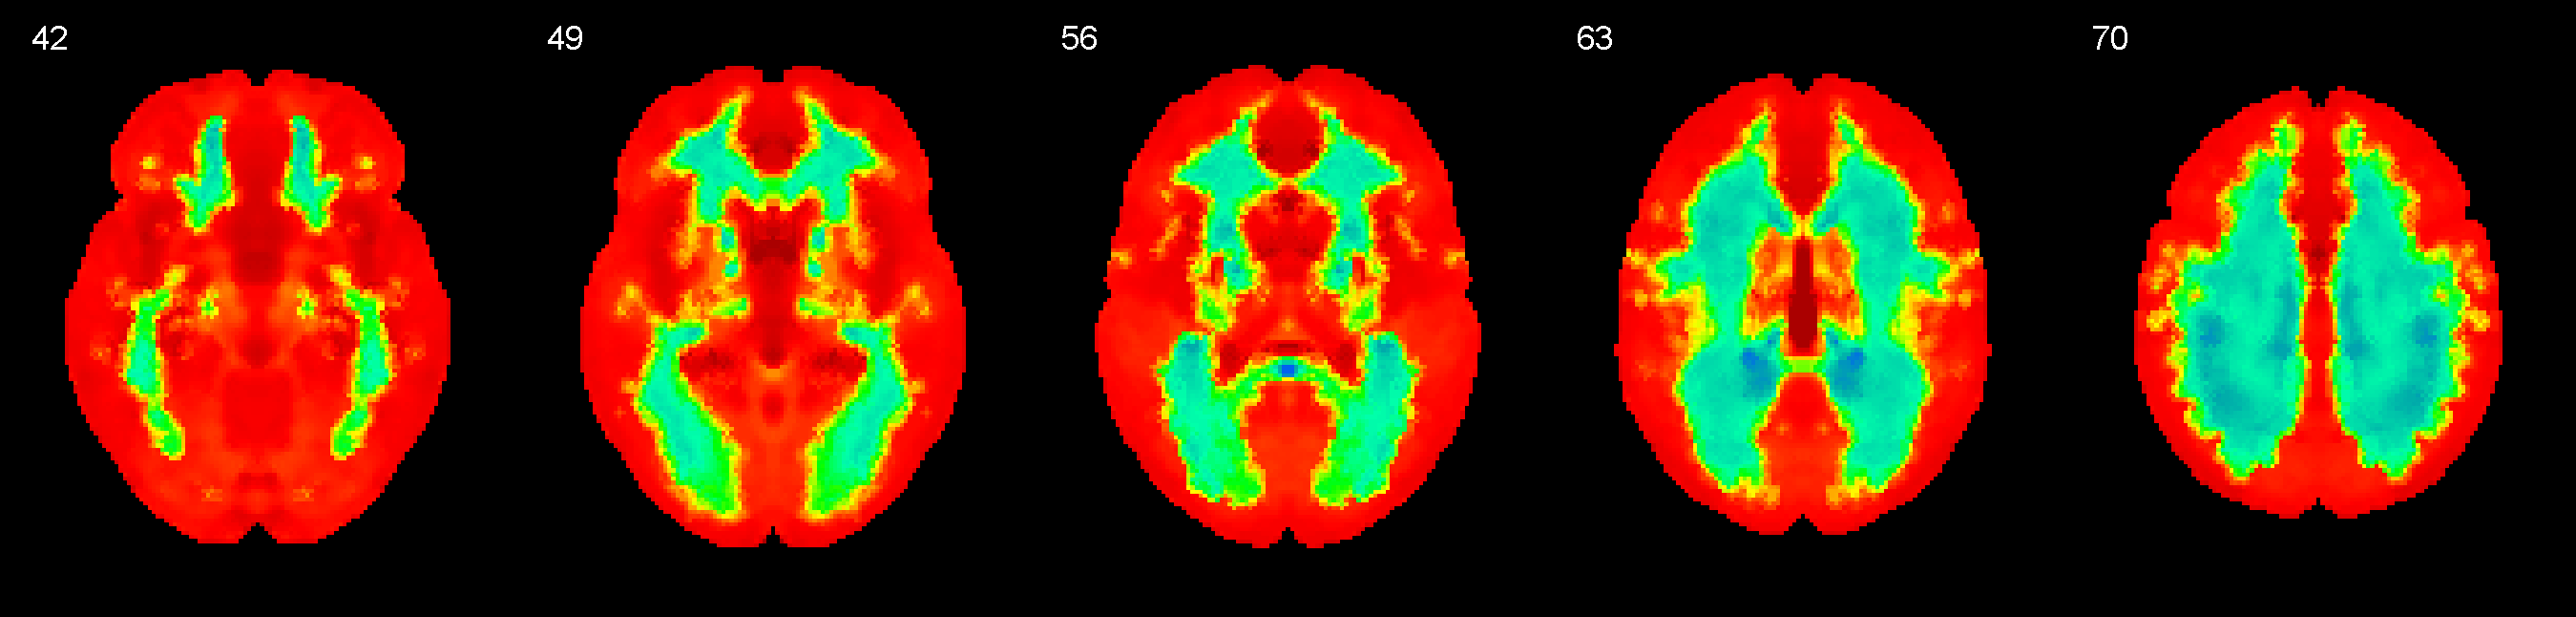
\includegraphics[height=\sliceheight]{T-r1.png}
    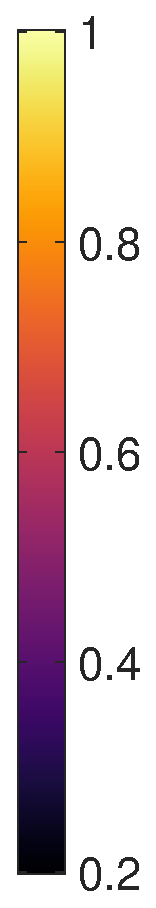
\includegraphics[height=\sliceheight]{cmap-r-T}%
  }\\[0.5em]
  \subfigureoverl[white]{$\mathcal{T}_{\mathrm{r}}(x)$}{}{%
    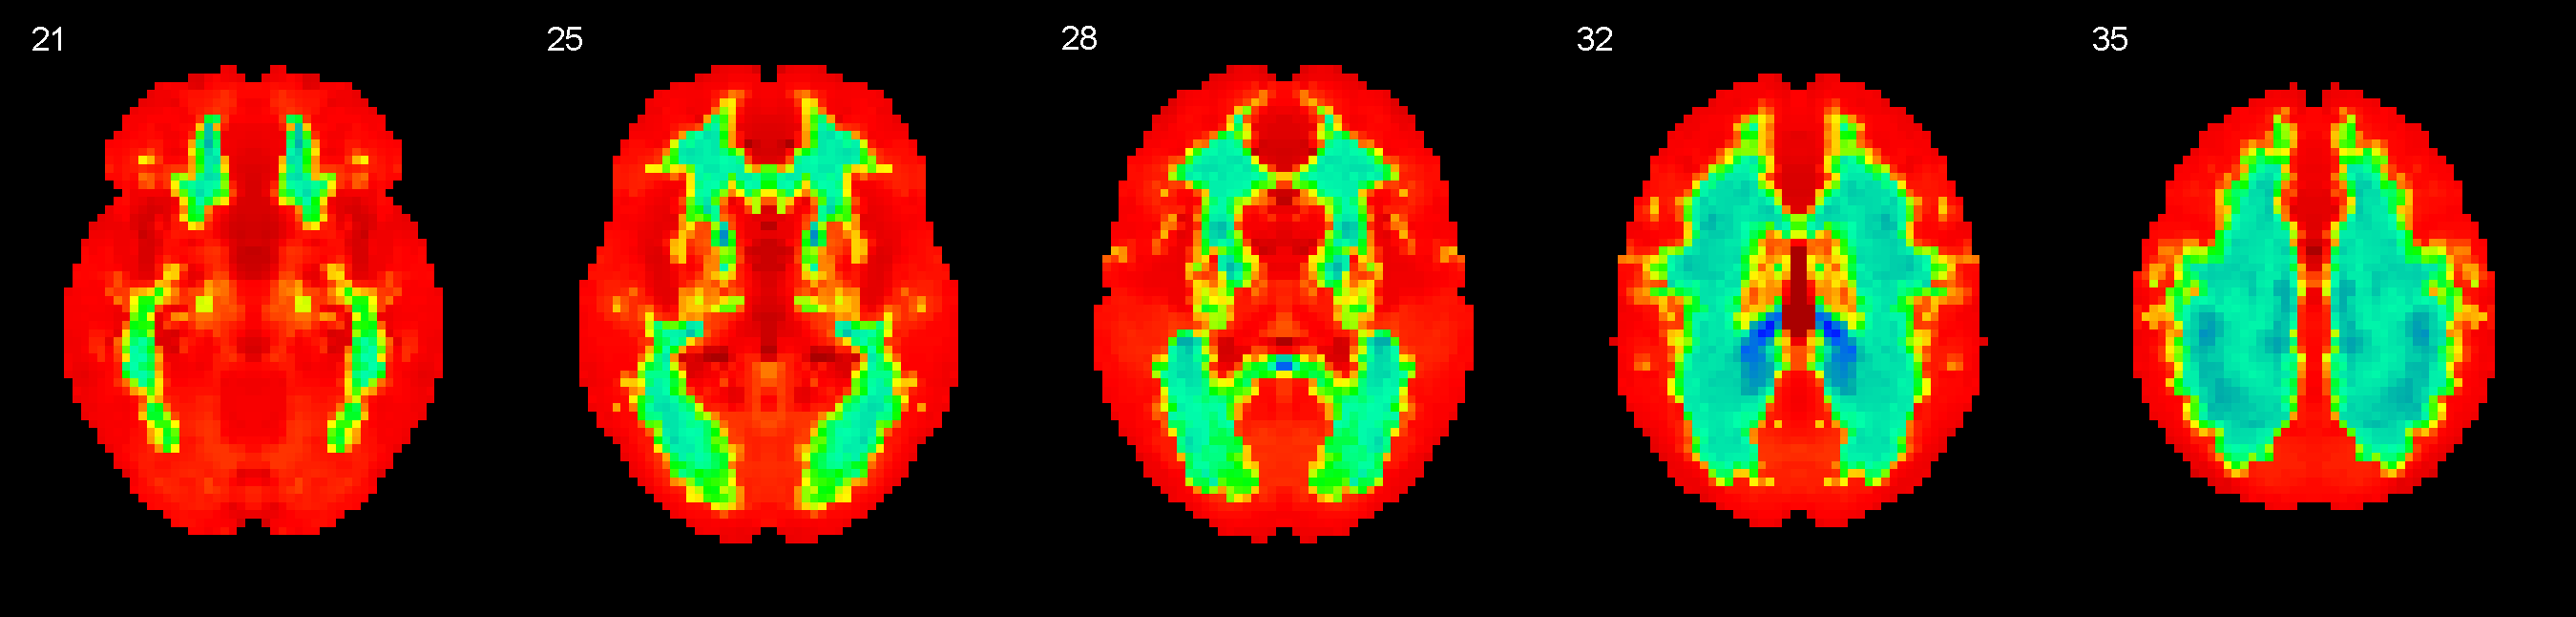
\includegraphics[height=\sliceheight]{T-r2.png}
    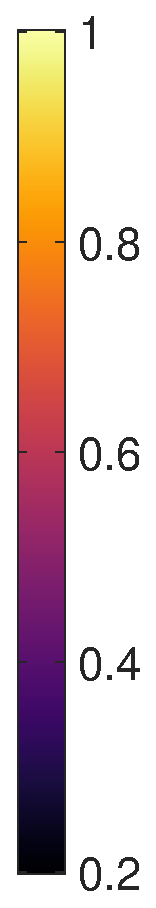
\includegraphics[height=\sliceheight]{cmap-r-T}%
  }\\[0.5em]
  \subfigureoverl[white]{$\mathcal{S}(x)$}{}{%
    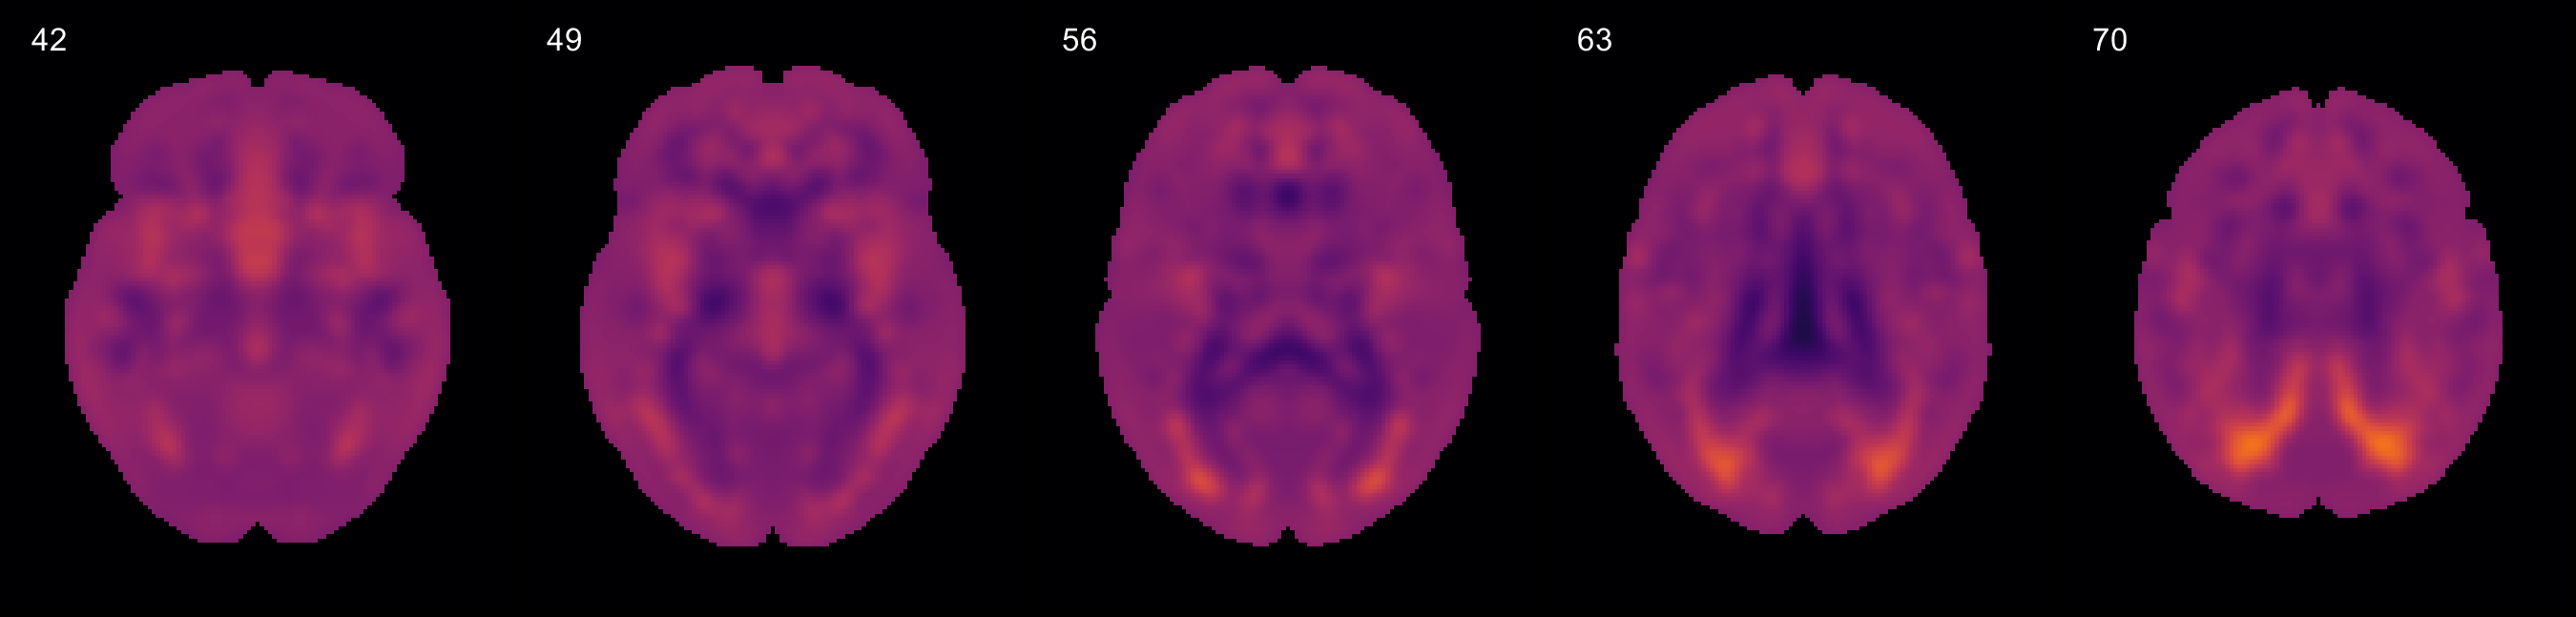
\includegraphics[height=\sliceheight]{S-r1.png}
    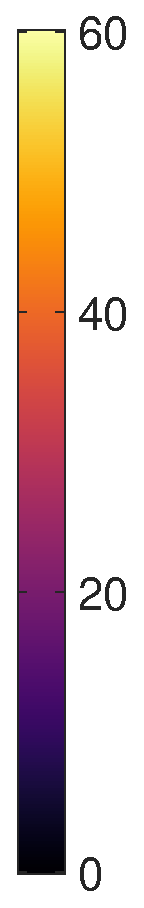
\includegraphics[height=\sliceheight]{cmap-r-S}%
  }\\[0.5em]
  \subfigureoverl[white]{$\mathcal{S}_{\mathrm{r}}(x)$}{}{%
    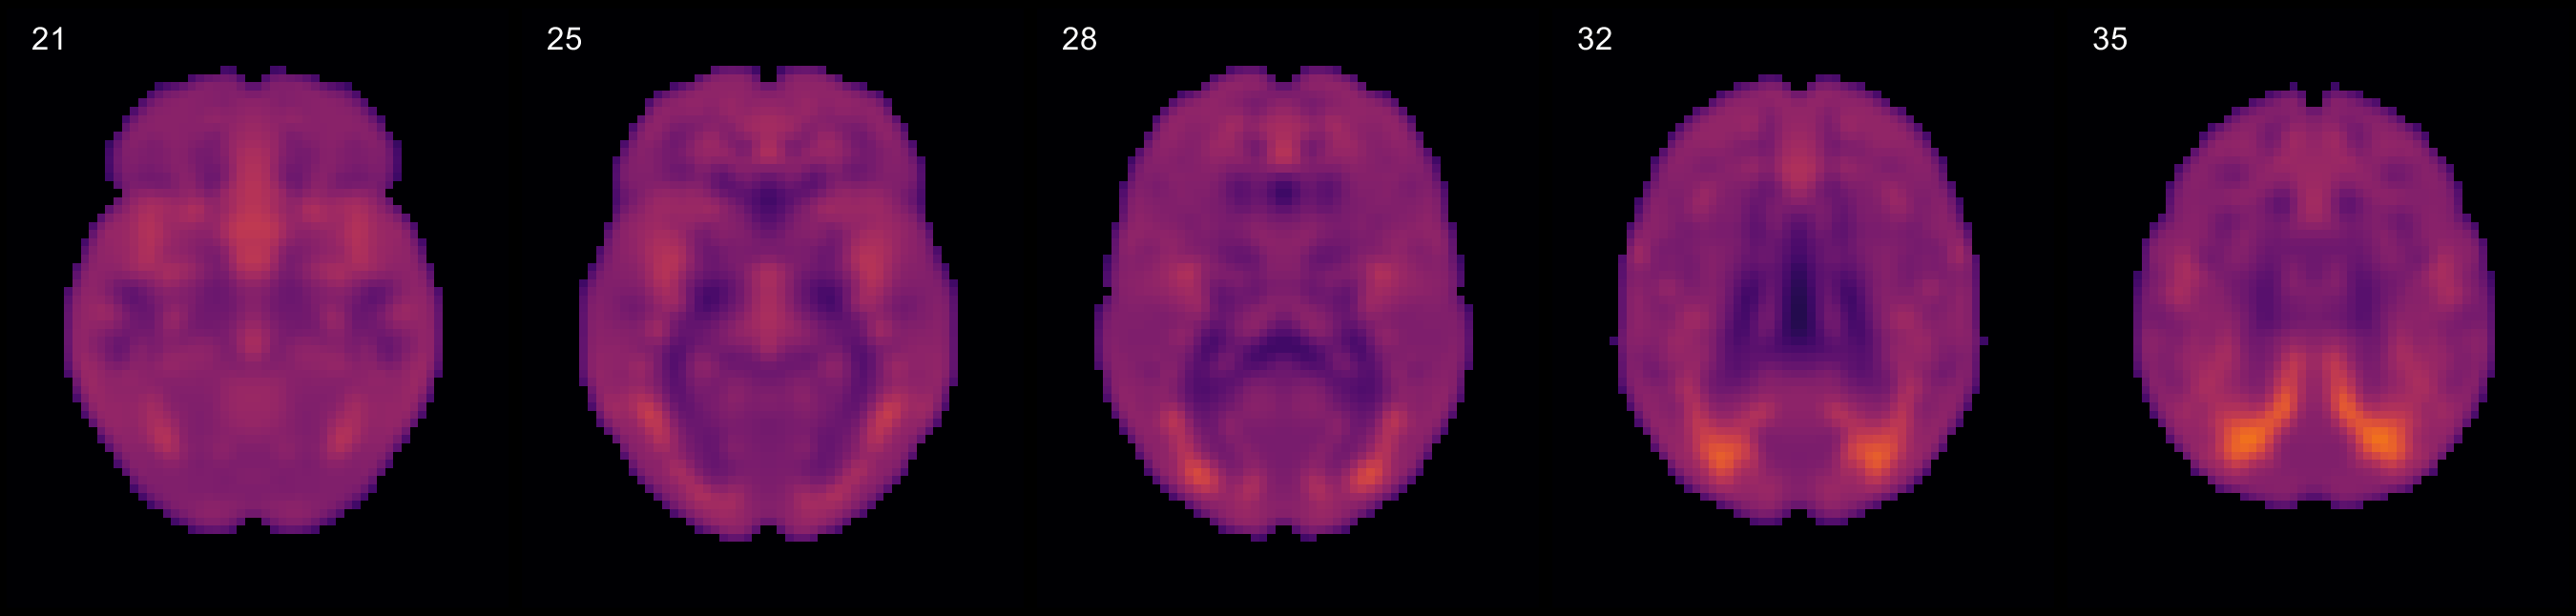
\includegraphics[height=\sliceheight]{S-r2.png}
    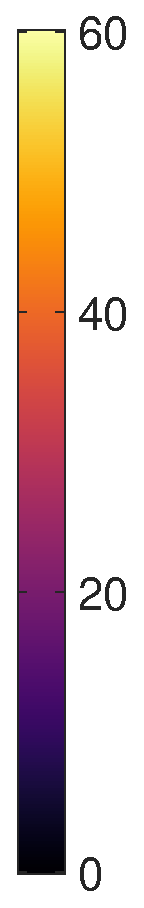
\includegraphics[height=\sliceheight]{cmap-r-S}%
  }\\[0.5em]
  \caption{Comparison of parameter images estimated at full and half-resolution.
  Best viewed in colour.}%
  \label{fig:beta-r}
\end{figure}
All results were computed with this adaptation (specifically $\mathrm{r} = 0.5$)
except for the parameter image smoothing experiments described in \S~\ref{sss:exp-beta-smooth},
which justify this modification.
% --------------------------------------------------------------------------------------------------
% ==================================================================================================
%%%%%%%%%%%%%%%%%%%%%%%%%%%%%%%%%%%%%%%%%%%%%%%%%%%%%%%%%%%%%%%%%%%%%%%%%%%%%%%%%%%%%%%%%%%%%%%%%%%%
